\documentclass[nooutcomes]{ximera}
\input{../preamble.tex}


\author{Elizabeth Miller}
%\license{Creative Commons 4.0 International License}



\title{Relations and Graphs: Famous Functions}

\begin{document}

\begin{abstract}
We list important relations and functions that will be explored throughout this course and used often in Calculus.
\end{abstract}
\maketitle

%\typeout{************************************************}
%\typeout{Famous Functions and Relations}
%\typeout{************************************************}

%\section{Famous Functions and Relations} 
Throughout this course and in Calculus you will study certain relations in depth.  These relations are usually functions, and they are the functions that come up often in real world applications.  In this section, we will give you a list of some of these functions, including their formula, their graph, and a table of some of their most important values.  You might not recognize some of these functions or know what their forumlas mean.  That is ok.  We will learn more about them throughout this course.  Remember, though, that a relation or function can be given by a graph.  For now, familiarize yourself with these graphs.  They will come up in examples throughout the course.

\begin{MM}
Eek! What am I supposed to do with all the information in this section? We know there's a lot of information here. First, bookmark this section so you can refer back to it. Throughout the course, you'll interact with these functions often. Over time, you'll be able to recall the information in this section without looking it up. But don't just  memorize the information. Remember to make connections between the formulas, graphs, and tables. For example, what does the formula tell you about the graph? Or the table tell you about the formula?

\end{MM}

\newpage

%\typeout{************************************************}
%\typeout{Linear Functions}
%\typeout{************************************************}

\section{Linear Functions}
Of the most important types of functions is a linear function. The graph of a linear function is a line.  

A prototypical example of a linear function

\begin{image}
  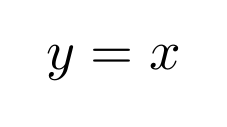
\begin{tikzpicture}[scale=2,every node/.style={transform shape}]
    \node at (0,0) {$y=x$};
  \end{tikzpicture}
\end{image}

\begin{image}
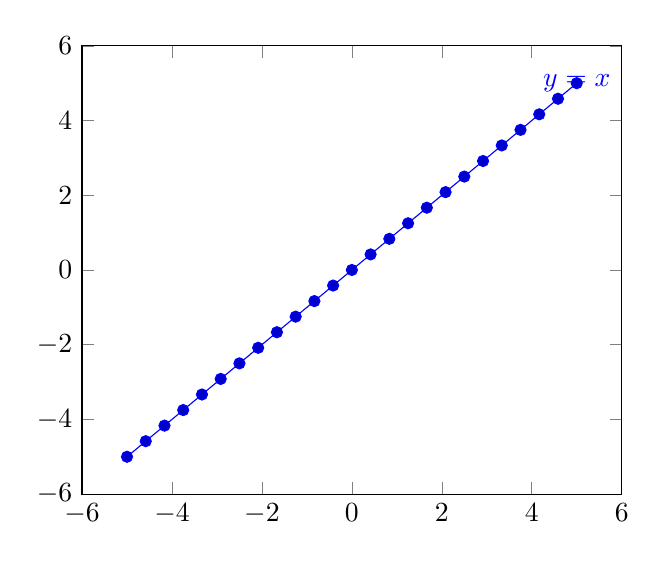
\begin{tikzpicture}
    \begin{axis}
        \addplot{x} node{$y=x$};
    \end{axis}
\end{tikzpicture}
\end{image}


\[
\begin{array}{  c  }
 %\hline
\text{\textbf{ Important Values of $y=x$}} \\
 \begin{array}{|c|c|}
 \hline
 x & y\\
 \hline
 -2&-2\\
 -1&-1\\
 0&0\\
 1&1\\
 2&2\\
 \hline
\end{array}
\end{array}
\]

In general, linear functions can be written as $y=mx+b$ where $m$ and $b$ can be any numbers.  You can play with changing the values of $m$ and $b$ on the graph using Desmos and see how that changes the line.  

\begin{center}  
\desmos{japnhapzvn}{800}{600}  
\end{center}


\newpage

%\typeout{************************************************}
%\typeout{Quadratic Functions}
%\typeout{************************************************}

\section{Quadratic Functions}

The graph of a quadratic function is a parabola.

A prototypical example of a quadratic function is 

\begin{image}
  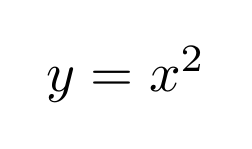
\begin{tikzpicture}[scale=2,every node/.style={transform shape}]
    \node at (0,0) {$y=x^2$};
  \end{tikzpicture}
\end{image}

\begin{image}
\begin{tikzpicture}
    \begin{axis}
        \addplot[smooth]{x^2} node{$y=x^2$};
    \end{axis}
\end{tikzpicture}
\end{image}

\[
\begin{array}{c }
\text{\textbf{Important Values of $y=x^2$}} \\
\begin{array}{|c|c|}
 \hline
 x & y\\
 \hline
 -2&4\\
 -1&1\\
 0&0\\
 1&1\\
 2&4\\
 \hline
\end{array}
\end{array}
\]

In general, quadratic functions can be written as $y=ax^2+bx+c$ where $a$, $b$, and $c$ can be any numbers.  You can play with changing the values of $a$, $b$, and $c$ on the graph using Desmos and see how that changes the parabola.  

\begin{center}  
\desmos{nmlghfrws9}{800}{600}  
\end{center}


\newpage

%\typeout{************************************************}
%\typeout{Absolute Value}
%\typeout{************************************************}

\section{Absolute Value Function}
The absolute value function takes all $y$-values and makes them positive.  The absolute value function is written as 

\begin{image}
  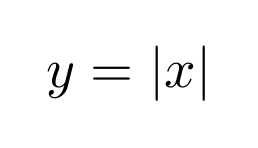
\begin{tikzpicture}[scale=2,every node/.style={transform shape}]
    \node at (0,0) {$y=|x|$};
  \end{tikzpicture}
\end{image}

\begin{image}
\begin{tikzpicture}
    \begin{axis}
        \addplot[smooth]{abs(x)} node{$y=|x|$};
    \end{axis}
\end{tikzpicture}
\end{image}

\[
\begin{array}{c }
\text{\textbf{Important Values of $y=|x|$}} \\
\begin{array}{|c|c|}
 \hline
 x & y\\
 \hline
 -2&2\\ 
-1&1\\ 
0&0\\
 1&1\\
 2&2\\
 \hline
\end{array}
\end{array}
\]



\newpage

%\typeout{************************************************}
%\typeout{Square Root}
%\typeout{************************************************}

\section{Square Root Function}
The square root function is written as

\begin{image}
  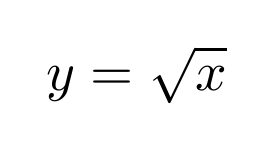
\begin{tikzpicture}[scale=2,every node/.style={transform shape}]
    \node at (0,0) {$y=\sqrt{x}$};
  \end{tikzpicture}
\end{image}

\begin{image}
\begin{tikzpicture}
    \begin{axis}
        \addplot[samples=200,domain=0:30]{sqrt(x)};
    \end{axis}
\end{tikzpicture}
\end{image}


\[
\begin{array}{c }
 \text{\textbf{ Important Values of $y=\sqrt{x}$}} \\
\begin{array}{|c|c|}
 \hline
 x & y\\
 \hline
 0&0\\
 1&1\\
 4&2\\
 9&3\\
 25&5\\
 \hline
\end{array}
\end{array}
\]



\newpage

%\typeout{************************************************}
%\typeout{Exponential}
%\typeout{************************************************}

\section{Exponential Functions}
The exponential growth function is written as

\begin{image}
  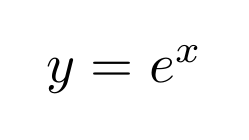
\begin{tikzpicture}[scale=2,every node/.style={transform shape}]
    \node at (0,0) {$y=e^{x}$};
  \end{tikzpicture}
\end{image}

Here $e$ is the mathematical constant known as Euler's number.  $e \approx 2.71828 .$.

\begin{image}
\begin{tikzpicture}
    \begin{axis}
        \addplot[samples=200,domain=-10:4]{e^x};
    \end{axis}
\end{tikzpicture}
\end{image}

\[
\begin{array}{c}
 \text{\textbf{Important Values of $y=e^x$}} \\
\begin{array}{|c|c|}
\hline
 x & y \\
 \hline 
 0&1\\[2ex]
 1&e\\[2ex]
 -1&e^{-1}=\frac{1}{e}\\[2ex]
\hline
\end{array}
\end{array}
 \]

In general, we can talk about exponential functions of the form $y=b^{x}$ where $b$ is a positive number not equal to $1$.  You can play with changing the values of $b$ on the graph using Desmos and see how that changes the graph.  Pay particular attention to the difference between $b>1$ and $0<b<1$.

\begin{center}  
%\desmos{dgcwh0chfv}{800}{600}  
\desmos{qsmvb7tiex}{800}{600}
\end{center}




\newpage

%\typeout{************************************************}
%\typeout{Logarithms}
%\typeout{************************************************}

\section{Logarithm Functions}


The most famous logarithm function is
\begin{image}
  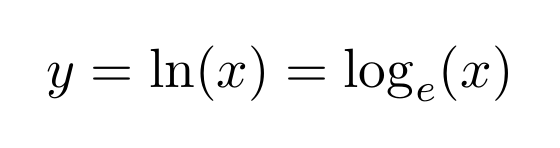
\begin{tikzpicture}[scale=2,every node/.style={transform shape}]
    \node at (0,0) {$y=\ln(x)=\log_{e}(x)$};
  \end{tikzpicture}
\end{image}
 
Here $e$ is the mathematical constant known as Euler's number. $e \approx 2.71828$.

\begin{image}
\begin{tikzpicture}
    \begin{axis}
        \addplot[samples=200,domain=0.01:8]{ln(x)};
    \end{axis}
\end{tikzpicture}
\end{image}



\[
\begin{array}{ c  }
% \hline
  \text{\textbf{Important Values of $y=\ln(x)$}}\\
 \begin{array}{|c|c|}
 \hline
 x & y\\
 \hline
0&\text{undefined}\\[2ex]
\frac{1}{e}&-1\\[2ex]
1&0\\[2ex]
e&1\\[2ex]
 \hline
 \end{array}
\end{array}
 \]


You may notice that the table of values for $y=\ln(x)$ and $y=e^x$ are similiar.  This is becase these two functions are interconnected.  We will explore this more later in the course.



In general, we can talk about logarithmic functions of the form $y=\log_b(x)$ where $b$ is a positive number not equal to $1$.  You can play with changing the values of $b$ on the graph using Desmos and see how that changes the graph.  Pay particular attention to the difference between $b>1$ and $0<b<1$.

\begin{center}  
\desmos{lxllnpdi6w}{800}{600}  
\end{center}



\newpage

%\typeout{************************************************}
%\typeout{Sine}
%\typeout{************************************************}

\section{Sine}
The sine function is written as

\begin{image}
  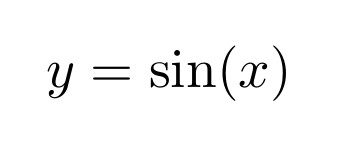
\begin{tikzpicture}[scale=2,every node/.style={transform shape}]
    \node at (0,0) {$y=\sin(x)$};
  \end{tikzpicture}
\end{image}


This function comes from trigonometry. In the table below we will use another mathematical constant, $\pi$ (``pi" pronounced pie). $\pi \approx 3.14159$.

\begin{image}
\begin{tikzpicture}
    \begin{axis}[ymin=-2, ymax=2,
		   %xtick={-6.28318, -4.7123889, -3.14159, -1.5708, 1.5708, 3.14159, 4.7123889, 6.28318},
    xticklabels={
        $-\frac{3\pi}{2}$, $-\pi$, $\frac{\pi}{2}$, $0$,
        $\frac{\pi}{2}$, $\pi$, $\frac{3\pi}{2}$, $2\pi$
    }, ]
        \addplot[samples=200]{sin(pi/4*deg(x))};
    \end{axis}
\end{tikzpicture}
\end{image}

\[
\begin{array}{ c }
 \text{ Important Values of  $y=\sin(x)$}\\
\begin{array}{|c|c|}
 \hline
 x & y\\
 \hline
 -\pi&0\\[2ex]
 -\frac{\pi}{2}&-1\\[2ex]
 0&0\\[2ex]
 \frac{\pi}{2}&1\\[2ex]
 \pi&0\\[2ex]
\frac{3\pi}{2}&-1\\[2ex]
 2 \pi&0\\[2ex]
\hline
\end{array}
\end{array}
\]


In general, we can consider $y=a\sin(bx)$.  You can play with changing the values of $a$ and $b$ on the graph using Desmos and see how that changes the graph.  

\begin{center}  
\desmos{vkxzcfv2aq}{800}{600}  
\end{center}

\end{document}
